In conjunction with the \pointer software, we can finally turn to the
main topic of interest in this Chapter: how can we accurately and
systematically develop intermolecular force fields? As discussed at the
beginning of \cref{ch:workflow},
with \mastiff
some aspects of the force field development process remain an `art', and are thus
usually guided by chemical intuition, whereas increasingly more aspects of force field
fitting now can be carried out in a systematic and reasonably black-box manner. Here
we offer an in-depth analysis of the force field development process for
\mastiff and related force fields, paying
specific attention to addressing both the `artistic' and `scientific' choices
that must be made when developing models for new systems. 

\begin{figure}
\centering
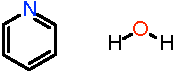
\includegraphics[width=0.3\textwidth]{pointer/molecules.pdf}
\caption{Pyridine and water -- molecular examples of challenges in force field fitting}
\label{fig:pointer-molecules}
\end{figure}

\begin{subsection}{General}

In general, a large number of development choices must be made prior to force field
fitting: which benchmark energies to use, how to sample the dimer \pes, which
parameters to treat as hard constraints, etc. While some of these choices have
been discussed in \cref{ch:workflow}, the following considerations also bear
mention:

\begin{paragraph}{Atom-typing}
In developing force fields for new systems (specifically with regards to the \mastiff approach, though
many of the principles below apply generally to other ab initio force fields),
an initial choice must be made as to how to categorize each atom into 
`atomtypes', where by definition all atoms within the same \atomtype share the
same force field functional form and parameters. In some cases, such as with
water, atomtyping is a fairly obvious decision, and it is easy to see how two
unique types should be used to describe the system. With other molecules
such as pyridine (\cref{fig:pointer-molecules}), however, this
atomtyping process is difficult to treat systematically and/or universally, and an iterative
guess-and-check process may be required to ascertain the number of atomtypes
that are required to obtain a desired level of force field accuracy (see
\cref{sec:pointer-exchange} for details).

Note that substantially increasing the number of free atomtypes (i.e., those
atomtypes whose parameters have not been pre-fit to a different system) 
can sometimes lead to numerical instabilities in fitting process or to
overfitting,\cite{Hawkins2004} and care must be taken with large/complex
systems to ensure good accuracy and transferability. 
\end{paragraph}

\begin{paragraph}{Anisotropy}
With the \mastiff approach, each atomtype can be treated as either
isotropic or anisotropic, and for anisotropic atoms an arbitrary number of
spherical harmonic terms can in principle be included in the functional form. These spherical
harmonic expansions are always calculated with respect to a user-defined local
atomic coordinate system, and this coordinate system should be chosen so as to
maximize the symmetry (or approximate symmetry) of the system (vida infra).

For anisotropic atomtypes, in addition to specifying a local coordinate system
it is necessary to specify the ranks and orders of included spherical harmonic
functions $\mathcal{C}_{lk}$ that get included in
\cref{eq:pointer-anisotropy}. In practice, inclusion of spherical harmonics
beyond rank $l=2$ does not typically lead to worthwhile accuracy gains, and we
suggest truncation at this order for most systems.  Additionally, na\"ive
inclusion of all spherical harmonics up to rank 2 can lead to numerical
instabilities, and so only symmetry-allowed spherical harmonics (based on the
local coordinate system) should be included.  With the \pointer code, these
specifications for anisotropy are listed in the .axes file, with notation as
in \cref{lst:pointer-axes}. 

For most atomtypes (see \cref{ch:mastiff} for details), an isotropic description of the system is
sufficient, and so anisotropy should typically only be necessary for
atomtypes corresponding or spatially proximate to heteroatoms and/or multiple
bonding environments. Still, it is always worthwhile to explicitly test the effects of treating
different atoms anisotropically via comparison to the \sapt exchange energy
(see \cref{sec:pointer-exchange} for details). 

\end{paragraph}

\begin{paragraph}{Benchmark Energies and Correction Factors}

In \cref{ch:lmoeda}, we have discussed situations in which a
\sapt-based energy decomposition may be insufficient for force field
development, and have suggested strategies for improvement in these cases. 
For most systems, however, a \sapt-based decomposition will be of good
accuracy, and any deviations between \sapt and gold-standard \ccsdt can be accounted for using a \dccsdt correction
term as in \cref{ch:mastiff}.
Preliminary results on \co, \cl, \ho, and \nh suggest that this \dccsdt term
should be included as part of the dispersion energy (see \cref{sec:pointer-dispersion}), however
more systems should be tested to see if this practice is appropriate for
general force field development.
\end{paragraph}

\end{subsection}
